\documentclass[12pt, a4paper]{article}
\usepackage{geometry}
\renewcommand{\baselinestretch}{1.0}
\usepackage[backend = biber, citestyle = authoryear, url = false]{biblatex}
\usepackage{hyperref}
\usepackage{pdflscape}
\usepackage{graphicx}
\addbibresource{sop.bib}
\title{Is small beautiful? Do small districts lead to better outcomes?}
\author{Jothsna Rajan \\
	\small{Indian Institute of Management, Bangalore, India}}
\geometry{a4paper, top=25mm}
\graphicspath{ {Images/} }
\usepackage{Sweave}
\begin{document}
\Sconcordance{concordance:seminar.tex:seminar.Rnw:%
1 13 1 1 0 131 1 1 15 1 1 1 4 44 0 1 3 1 16 40 0 1 23 39 0 1 2 1 13 40 %
0 1 23 39 0 1 2 1 11 15 1 1 16 40 0 1 21 39 0 1 3 1 16 40 0 1 22 39 0 1 %
2 1 15 34 0 1 7 46 0 1 7 46 0 1 7 46 0 1 2 3 5 2 1}

	\maketitle
	\begin{abstract}
		What is the optimal population level for local public service delivery? In the question over the optimal size of local government systems, small jurisdictions have been attributed a lot of merits. But does bifurcating larger districts into smaller ones pay off? I examine this question in the context of public education using data from a district bifurcation process in Karnataka, India. Performance of sub-districts which were allocated to newly created smaller districts is compared with sub-districts that remained in larger districts using a difference in difference estimation model. Education performance is measured in test scores, as well as inputs to schooling such as number of schools, funding to schools, academic inspections etc. The results seem to suggest that there is no significant improvement in education outcomes as a result of the bifurcation. 
	\end{abstract}
\paragraph{} Is there an optimal size for local government systems? Aristotle in his treatise `Politics' argued that political entities needed to balance the twin considerations of economic viability and effective citizenship \parencite{aristotle_politics_1984}. In modern democracies, debates on the topic are framed in a similar language with two sets of normative criteria. The first one is \textit{output legitimacy}. The function of local governments is to provide a set of public goods and services to its citizens and promote public welfare. A government that fulfils this duty better has higher output legitimacy. The other normative concern is `citizen effectiveness' or the capability and willingness of citizens to control the decisions made on their behalf \parencite{dahl_size_1973}. Enhancing citizen effectiveness raises the \textit{input legitimacy} of the system. Both output and input legitimacy are prerequisites to democratic legitimacy \parencite{scharpf_governing_1999}. The fundamental assumption in these debates is that changing the size of political units is likely to affect the democratic quality (input legitimacy) and functional effectiveness (output legitimacy) of governments. 

\paragraph{}  Recent debates on the topic attribute considerable virtues to small jurisdictions. In democratic societies, the economic and political arguments tend to converge. Small jurisdictions are believed to enhance political participation, make politics less abstract, politicians more responsive, and facilitate exit-based empowerment of citizens \parencite{hansen_size_2014}. Decentralisation will also increase economic efficiency as the local governments have an information advantage and can respond better to variance in preferences at the local level \parencite{oates_fiscal_1972}, and population mobility will lead to competition between local authorities and better provision of public goods. Decentralised service delivery especially when citizens directly elect the local governments is expected to provide better coverage, quality and efficiency \parencite{smoke2015rethinking}. Competing local governments may experiment with various ways to provide public goods and lead to innovations that can be applied elsewhere. These considerations suggest that public goods that are (1) sensitive to local preferences and (2) do not have large spillover (3) nor scale effects: infrastructure, public education, etc. are better provided under decentralisation (\cite{tiebout_economies_1960}, \cite{oates_fiscal_1972}). At the same time there is a counter argument in favour of larger jurisdiction sizes because it allows for economies of scale in the providing public goods \parencite{hirsch_expenditure_1959}. 

\paragraph{} In a bid to arrive at the optimal population size in a local government unit, many national governments have reorganized their sub-national boundaries. Europe has seen local government consolidation via municipal amalgamations while transitional economies have seen increasing decentralization at the local government level. Since the 1950s, India has seen frequent administrative bifurcations at the local government level (district level). The number of districts in the country has increased from 356 in the 1971 census period to 640 in the 2011 census (Table. \ref{Fig2}) This is a trend that is continuing in the present day. West Bengal has created five new districts since 2015. The rationale for creating of new districts was stated to be - ``...for \textit{better administrative control} and so that \textit{public service can be delivered at the door steps} of the people staying at remote areas'' (emphasis added) \parencite{Mamata}. Similarly, Telangana state is contemplating the creation of 14 - 15 new districts \parencite{Telengana} and Haryana state is considering 3 more districts \parencite{Haryana}. In all these cases, the stated rationale for district bifurcation is decentralisation of administration and better public service. And India is not alone in the implementation of administrative bifurcations at the local government level. Brazil, in the period from 1990 to 2000, increased the number of municipalities from 4,491 to 5,560 \parencite{tomio2005creation}. Russia adopted Local Government Reform in 2003 and since then has doubled the number of municipalities \parencite{turgel2008new}\nocite{avellaneda_is_2015}. But does creation of new districts enhance public service outcomes?

\paragraph{}This paper explores the impact of bifurcation of districts on the quality of public service delivery - specifically, the quality of public education. I present the theory behind reorganization and the available evidence on its effectiveness, and discuss the methodological challenges in the empirical examination of size effects. I test my propositions using data collected on public education in the districts of Karnataka in India over a 9 year period from 2005 to 2013. Karnataka created three new districts by bifurcating three existing ones during the period. Remaining districts were left untouched. A new district is created by reallocating some of the taluks (sub-districts) within an existing district to a new one. This allows use of a difference in difference model to test for the effect of the policy on education outcomes. The reform was driven by the state government, following public demand for creation of new districts and had taken place at different times. But the rationale for the public demand was based on cultural factors rather than public education concerns. 

\section*{Theory}
\paragraph{} The fundamental argument in favour of decentralized governance comes from the perspective that there is heterogeneity in demand for public services. The variance in demand can be better understood and catered to by a government that is closer to the citizens, thus raising well-being throughout society. Tiebout, in his 1956 paper, talks about citizens \textit{voting with their feet} or \textit{exiting}. He conceptualizes a fully mobile citizen that can move to a jurisdiction that matches her preferences for tax rates and public service levels, thus revealing her preferences \parencite{tiebout_economies_1960}. This information can then be used by local governments to tailor their own activities and thus raise welfare. But how much decentralization should we demand? Oates' Decentralization theorem formalizes it as \textit{``...in the absence of cost-savings from the centralized provision of a [local public] good and of interjurisdictional externalities, the level of welfare will always be at least as high (and typically higher) if Pareto-efficient levels of consumption are provided in each jurisdiction than if any single, uniform level of consumption is maintained across all jurisdictions''}(\cite{oates_fiscal_1972}, pg 54). \nocite{oates1999essay}

\paragraph{} In other words, a public good that does not have large economies of scale or inter-jurisdictional externalities may be better provided under decentralization. Public education is not seen as imposing strong externalities on neighbouring regions, nor does it have large scale effects. Therefore, under the classic explanation, a smaller district should be able to provide better service. At the same time, practical considerations remain. We might need to build administrative capacity when a larger district is split into two or more before any benefits can be reaped. Also, if the districts are too small in the first place, there might be some benefit in consolidating two or more districts and managing them together.  

\paragraph{Jurisdiction Size} Administrative bifurcations lead to lowering of the jurisdiction size and are often pursued in hopes that smaller population sizes will lead to administrative convenience and better allocative efficiency. Smaller populations may reduce agency costs especially if the local administrators are directly elected and also reduce information costs because of the proximity of the decision making centre to the citizens. It may also lead to lower costs in planning and monitoring activities than in a larger jurisdiction. Some of these effects are likely to materialize over a longer period of time and would require a long research period. On the other hand larger jurisdiction size will allow you to spread fixed costs of a greater population. Vito Tanzi offers an argument for corruption to be higher at local levels than at central government levels, because of closer interaction at the local level between the bureaucrats and citizens that can enable nepotism and personal favours \parencite{tanzi1996macroeconomic}. \nocite{allers2016effects} \nocite{lassen_jurisdiction_2011} The optimal jurisdiction size at which public service delivery begins to improve or decline might also be a function of the specific public good or service. It also needs to be stated that the effects of size on public service delivery depends on the size of production units as well, not just administrative units. For example, in the case of public education, a smaller district may recognize the need for higher educational spending and raise the number of schools in the region accordingly, but the educational outcomes or test scores would depend on the size and characteristics of the school as well. 

\paragraph{Service Levels} Local governments have a limited scope in varying service levels within their jurisdictions. If there is heterogeneity in preferences, it may be reflected in levels of public service delivered. A smaller administrative units allow for greater allocative efficiency of public budgets by allowing administrators to take preference heterogeneity into account. Conditional on the variation in preferences a district after bifurcation may exhibit divergence in service levels. If preferences are more homogeneous then there will be less need to deviate from previous service levels. 
\paragraph{} There is evidence from the decentralisation reforms in Bolivia and Columbia to suggest that decentralisation has enhanced the local allocative efficiency of public funds. Notably, it has resulted in shifting resources towards education in regions where education performance has historically been worse. But data limitations prevent the authors from testing whether the improvement extends to education outcomes, such as literacy and test scores \parencite{faguet2008decentralization}. Also, there is evidence from California state, to suggest that students in smaller districts perform better than those in larger districts in standardised tests after controlling for a variety of other factors \parencite{driscoll2003school}. The effect of either of these policies - bifurcation or consolidation (or a combination of both) - depends on the particular context and capabilities of the local administrative body. Holzer et al in 2009 provide a review of the empirical literature on this question. Their review suggests that the evidence on the effect of size on local government performance is inconclusive - there is very little correlation between size and efficiency for population sizes between 25,000 and 250,000 - anything above that or below is less efficient \parencite{holzer2009literature}. Decentralization at the local government level is a step that is frequently taken - despite the lack of strong evidence in its favour. 

\paragraph{} The critics of decentralisation argue that the its effectiveness is often greatly hampered by the particular context of its implementation.  Also, local bureaucracies may be poorly staffed and ill-equipped to handle the responsibilities associated with the decentralised provision of public goods \parencite{prud1995dangers}. The precise nature of decentralisation, such as the financial autonomy of the local government may also pay a role in determining whether the benefits can be reaped. These factors caution against the implementation of decentralisation as a panacea for administrative ills. It also means that any instance of decentralisation can be explored further to understand the context of success or failure.

\section*{Endogeneity Problem}
\paragraph{} Spatial and temporal variation in public policy affords the conditions suitable for identifying the impact of the policy on outcomes. But the size and boundary of the administrative unit is an active response to a problem and is endogenous - it can be included in the left \textit{or} right side of the estimation equation. In this paper I estimate the effect of the bifurcation of the administrative district on the public spending and quality of educational service delivered in the district. The identification is complicated by the fact the districts that were not split may be different from those that were. The demand for creation a new district usually arises from within the district, and the political traction gained by the idea has a role to play in the eventual decision made by the state. If the source of variation in policy action arises from within the characteristics of the intended beneficiaries of policy, then we have a policy endogeneity. Policy variation itself may be an outcome of some other characteristics. 
\section*{Methodology}
\paragraph{} At the 2001 census, Karnataka state had 27 districts - each with an average population of over 660,000 (If we exclude the urban district of Bangalore, the average drops to around 470,000). In the last decade Karnataka state in the south of India carved out three new districts from three existing ones. Two new districts (Chikballapura and Ramanagara) were created from two existing ones (Kolar and Bangalore rural respectively) in 2007, and a third new district (Yadgir) was created from an existing one (Gulbarga) in 2010 taking the total in the state up to 30. Creation of a new district entails additional administrative costs as the new districts often need to create the administrative infrastructure.


%\section*{Results}
%\section*{Discussion}
%\section*{Conclusion}
%\section*{Future Plans}
\printbibliography
\section*{Appendix}
\begin{table}[h!]
	\centering
	\caption{New Districts created in India - Statewise}
	\label{Fig1}
	\begin{tabular}{c|cccc} 
		\hline
		States/UTs & 1971-81 & 1981-91 & 1991-2001 & 2001-11 \\
		\hline 
		Andaman and Nicobar Islands & 1 & 0 & 0 & 1  \\ 
		Andhra Pradesh & 2 & 0 & 0 & 0  \\ 
		Arunachal Pradesh & 4 & 2 & 2 & 3  \\ 
		Assam & 0 & 13 & 0 & 4  \\ 
		Bihar & 14 & 11 & 8 & 1  \\ 
		Chhattisgarh & 0 & 0 & 9 & 2  \\ 
		Daman and Diu & 0 & 2 & 0 & 0  \\ 
		Delhi & 0 & 0 & 8 & 0  \\ 
		Goa & 0 & -1 & 0 & 0  \\ 
		Gujarat & 0 & 0 & 6 & 1  \\ 
		Haryana & 5 & 4 & 3 & 2  \\ 
		Himachal Pradesh & 2 & 0 & 0 & 0  \\ 
		Jammu and Kashmir & 4 & 0 & 0 & 8  \\ 
		Jharkhand & 0 & 0 & 5 & 6  \\ 
		Karnataka & 0 & 1 & 7 & 3  \\ 
		Kerala & 2 & 2 & 0 & 0  \\ 
		Madhya Pradesh & 2 & 0 & 7 & 5  \\ 
		Maharashtra & 0 & 4 & 5 & 0  \\ 
		Manipur & 1 & 2 & 1 & 0  \\ 
		Meghalaya & 3 & 0 & 2 & 0  \\ 
		Mizoram & 3 & 0 & 5 & 0  \\ 
		Nagaland & 4 & 0 & 1 & 3  \\ 
		Odisha & 0 & 0 & 17 & 0  \\ 
		Punjab & 1 & 0 & 5 & 3  \\ 
		Rajasthan & 0 & 1 & 5 & 1  \\ 
		Tamil Nadu & 2 & 5 & 9 & 2  \\ 
		Tripura & 0 & 0 & 1 & 0  \\ 
		Uttar Pradesh & 2 & 7 & 16 & 1  \\ 
		Uttarakhand & 0 & 0 & 4 & 0  \\ 
		West Bengal & 0 & 1 & 1 & 1  \\ 
		\hline
		Overall & 52 & 54 & 127 & 47  \\ 
		\hline
	\end{tabular}
\end{table}

\begin{table}[h!]
	\centering
	\caption{No\# of Districts in India - Statewise}
	\label{Fig2}
	\begin{tabular}{c|ccccc} 
		\hline
		States/UTs & 1971 & 1981 & 1991 & 2001 & 2011 \\
		\hline 
		Andaman \& Nicobar Islands & 1 & 2 & 2 & 2 & 3 \\ 
		Andhra Pradesh & 21 & 23 & 23 & 23 & 23 \\ 
		Arunachal Pradesh & 5 & 9 & 11 & 13 & 16 \\ 
		Assam & 10 & 10 & 23 & 23 & 27 \\ 
		Bihar & 17 & 31 & 42 & 37 & 38 \\ 
		Chandigarh & 1 & 1 & 1 & 1 & 1 \\ 
		Chhattisgarh &  &  &  & 16 & 18 \\ 
		Dadra \& Nagar Haveli & 1 & 1 & 1 & 1 & 1 \\ 
		Daman \& Diu &  &  & 2 & 2 & 2 \\ 
		Delhi & 1 & 1 & 1 & 9 & 9 \\ 
		Goa & 3 & 3 & 2 & 2 & 2 \\ 
		Gujarat & 19 & 19 & 19 & 25 & 26 \\ 
		Haryana & 7 & 12 & 16 & 19 & 21 \\ 
		Himachal Pradesh & 10 & 12 & 12 & 12 & 12 \\ 
		Jammu \& Kashmir & 10 & 14 & 14 & 14 & 22 \\ 
		Jharkhand &  &  &  & 18 & 24 \\ 
		Karnataka & 19 & 19 & 20 & 27 & 30 \\ 
		Kerala & 10 & 12 & 14 & 14 & 14 \\ 
		Lakshadweep & 1 & 1 & 1 & 1 & 1 \\ 
		Madhya Pradesh & 43 & 45 & 45 & 45 & 50 \\ 
		Maharashtra & 26 & 26 & 30 & 35 & 35 \\ 
		Manipur & 5 & 6 & 8 & 9 & 9 \\ 
		Meghalaya & 2 & 5 & 5 & 7 & 7 \\ 
		Mizoram &  & 3 & 3 & 8 & 8 \\ 
		Nagaland & 3 & 7 & 7 & 8 & 11 \\ 
		Orissa & 13 & 13 & 13 & 30 & 30 \\ 
		Pondicherry & 4 & 4 & 4 & 4 & 4 \\ 
		Punjab & 11 & 12 & 12 & 17 & 20 \\ 
		Rajasthan & 26 & 26 & 27 & 32 & 33 \\ 
		Sikkim & 4 & 4 & 4 & 4 & 4 \\ 
		Tamil Nadu & 14 & 16 & 21 & 30 & 32 \\ 
		Tripura & 3 & 3 & 3 & 4 & 4 \\ 
		Uttar Pradesh & 54 & 56 & 63 & 70 & 71 \\ 
		Uttaranchal &  &  &  & 13 & 13 \\ 
		West Bengal & 16 & 16 & 17 & 18 & 19 \\ 
		\hline
		States & 19 & 22 & 25 & 29 &  \\ 
		Union Territories & 10 & 9 & 7 & 6 &  \\ 
		Districts & 356 & 412 & 466 & 593 & 640 \\ 
		\hline
	\end{tabular}
\end{table}


\begin{landscape}
% Table created by stargazer v.5.2 by Marek Hlavac, Harvard University. E-mail: hlavac at fas.harvard.edu
% Date and time: Wed, Jul 13, 2016 - 11:54:53 AM
\begin{table}[!htbp] \centering 
  \caption{No of Schools District-wise, across the years} 
  \label{} 
\footnotesize 
\begin{tabular}{@{\extracolsep{5pt}} ccccccccccc} 
\\[-1.8ex]\hline 
\hline \\[-1.8ex] 
 & District & Yr2005 & Yr2006 & Yr2007 & Yr2008 & Yr2009 & Yr2010 & Yr2011 & Yr2012 & NA. \\ 
\hline \\[-1.8ex] 
1 & BAGALKOT & $229$ & $255.0$ & $265.0$ & $269.0$ & $277.0$ & $281$ & $340.0$ & $291.0$ & $292.0$ \\ 
2 & BANGALORE RURAL & $330$ & $324.0$ & $330$ & $328.0$ & $332.0$ & $330.0$ & $367.0$ & $340.0$ & $343.0$ \\ 
3 & BELGAUM & $260$ & $277.0$ & $269.0$ & $283$ & $285.0$ & $291.0$ & $366.0$ & $304.0$ & $304.0$ \\ 
4 & BELGAUM CHIKKODI & $337.0$ & $358.0$ & $291$ & $307.0$ & $320.0$ & $324.0$ & $383.0$ & $328.0$ & $332.0$ \\ 
5 & BELLARY & $213.0$ & $224.0$ & $228$ & $231.0$ & $232$ & $240.0$ & $290.0$ & $246.0$ & $244.0$ \\ 
6 & BIDAR & $262.0$ & $290$ & $322.0$ & $336.0$ & $358.0$ & $377.0$ & $471.0$ & $399.0$ & $414.0$ \\ 
7 & BIJAPUR & $326.0$ & $336.0$ & $327$ & $336.0$ & $345$ & $366$ & $439$ & $392.0$ & $396$ \\ 
8 & CHAMARAJANAGARA & $310$ & $254$ & $180$ & $184.0$ & $186$ & $188.0$ & $229.0$ & $189.0$ & $188.0$ \\ 
9 & CHIKKABALLAPURA & $307.0$ & $295.0$ & $300$ & $309.0$ & $312.0$ & $313.0$ & $357$ & $321.0$ & $319.0$ \\ 
10 & CHIKKAMANGALORE & $253.0$ & $261.0$ & $235.0$ & $224.0$ & $218.0$ & $221.0$ & $258$ & $223.0$ & $225.0$ \\ 
11 & CHITRADURGA & $309.0$ & $310.0$ & $315$ & $330.0$ & $332.0$ & $335.0$ & $398$ & $340$ & $342$ \\ 
12 & DAKSHINA KANNADA & $218.0$ & $223.0$ & $226.0$ & $229$ & $231.0$ & $232.0$ & $294.0$ & $234$ & $235.0$ \\ 
13 & DAVANAGERE & $262.0$ & $268.0$ & $274.0$ & $273.0$ & $275.0$ & $278.0$ & $346.0$ & $279.0$ & $282.0$ \\ 
14 & DHARWAD & $197.0$ & $207.0$ & $145$ & $148.0$ & $153.0$ & $149.0$ & $185.0$ & $152$ & $156.0$ \\ 
15 & GADAG & $128.0$ & $131$ & $135.0$ & $135.0$ & $138.0$ & $141.0$ & $183$ & $146$ & $145.0$ \\ 
16 & GULBARGA & $244.0$ & $252.0$ & $262$ & $283$ & $290.0$ & $300.0$ & $365.0$ & $322.0$ & $326.0$ \\ 
17 & HASSAN & $364.0$ & $367$ & $365$ & $367.0$ & $366.0$ & $371.0$ & $428.0$ & $362.0$ & $363.0$ \\ 
18 & HAVERI & $171.0$ & $176.0$ & $180.0$ & $187.0$ & $191.0$ & $195.0$ & $242.0$ & $199.0$ & $200.0$ \\ 
19 & KODAGU & $168$ & $172.0$ & $173.0$ & $178.0$ & $178.0$ & $178.0$ & $226.0$ & $179$ & $181.0$ \\ 
20 & KOLAR & $421$ & $437.0$ & $419$ & $402.0$ & $403.0$ & $405.0$ & $449.0$ & $406.0$ & $404$ \\ 
21 & KOPPAL & $265$ & $271$ & $288$ & $292.0$ & $297.0$ & $305.0$ & $369.0$ & $325.0$ & $334$ \\ 
22 & MANDYA & $294.0$ & $295.0$ & $296.0$ & $298$ & $296.0$ & $298.0$ & $344.0$ & $302.0$ & $292.0$ \\ 
23 & MYSORE & $293.0$ & $301.0$ & $303.0$ & $307.0$ & $310.0$ & $315.0$ & $370$ & $316.0$ & $315.0$ \\ 
24 & RAICHUR & $294.0$ & $308$ & $324.0$ & $348.0$ & $361$ & $381$ & $445.0$ & $394.0$ & $402.0$ \\ 
25 & RAMANAGARA & $388.0$ & $386.0$ & $395.0$ & $396.0$ & $401$ & $406.0$ & $454.0$ & $391.0$ & $392.0$ \\ 
26 & SHIMOGA & $319.0$ & $317.0$ & $327.0$ & $329.0$ & $331.0$ & $333.0$ & $389.0$ & $335.0$ & $332$ \\ 
27 & TUMKUR & $436$ & $436$ & $445.0$ & $435.0$ & $436.0$ & $429$ & $496.0$ & $427.0$ & $423.0$ \\ 
28 & TUMKUR MADHUGIRI & $351$ & $346$ & $352.0$ & $352.0$ & $358.0$ & $362.0$ & $422$ & $363.0$ & $364.0$ \\ 
29 & UDUPI & $284.0$ & $283$ & $200$ & $192.0$ & $194.0$ & $194.0$ & $258.0$ & $196.0$ & $196.0$ \\ 
30 & UTTARA KANNADA & $212.0$ & $216.0$ & $215.0$ & $219.0$ & $219.0$ & $219.0$ & $249$ & $221.0$ & $221.0$ \\ 
31 & UTTARA KANNADA SIRSI & $200.0$ & $200.0$ & $203$ & $208$ & $209$ & $207.0$ & $234.0$ & $209$ & $209.0$ \\ 
32 & YADAGIRI & $298.0$ & $311.0$ & $328.0$ & $339.0$ & $358$ & $374.0$ & $441.0$ & $398$ & $404$ \\ 
\hline \\[-1.8ex] 
\end{tabular} 
\end{table} \end{landscape}
% Table created by stargazer v.5.2 by Marek Hlavac, Harvard University. E-mail: hlavac at fas.harvard.edu
% Date and time: Wed, Jul 13, 2016 - 11:54:53 AM
\begin{table}[!htbp] \centering 
  \caption{Summary Statistics in 2005} 
  \label{} 
\begin{tabular}{@{\extracolsep{5pt}} ccc} 
\\[-1.8ex]\hline 
\hline \\[-1.8ex] 
 & Undivided & Divided \\ 
\hline \\[-1.8ex] 
TotalMarks & $321.0$ & $302.0$ \\ 
Rural & $0.9$ & $0.9$ \\ 
WorkDays & $89.0$ & $102.0$ \\ 
AcadInsp & $0.5$ & $0.4$ \\ 
DevGrantR & $2,765.0$ & $2,592.0$ \\ 
DevGrantE & $1,641.0$ & $1,298.0$ \\ 
TLMGrantR & $3,537.0$ & $3,989.0$ \\ 
TLMGrantE & $1,763.0$ & $1,793.0$ \\ 
Classrooms & $4.0$ & $3.4$ \\ 
ToiletG & $1$ & $1$ \\ 
Electricity & $0.7$ & $0.5$ \\ 
Library & $0.8$ & $0.8$ \\ 
PlayGround & $0.6$ & $0.5$ \\ 
Male\_Tch & $2.4$ & $2.0$ \\ 
Female\_Tch & $2.0$ & $1.6$ \\ 
Grad\_Tch & $30.0$ & $26.0$ \\ 
ProfQ\_Tch & $4.2$ & $3.3$ \\ 
Days\_nonTch & $0.8$ & $1.9$ \\ 
Public & $0.9$ & $0.9$ \\ 
Split & $0$ & $1$ \\ 
Households & $49,571.0$ & $47,044.0$ \\ 
TotPop & $256,392.0$ & $247,430.0$ \\ 
Pop0.6 & $35,845.0$ & $36,113.0$ \\ 
Literates & $138,828.0$ & $120,988.0$ \\ 
TotWPop & $116,550.0$ & $117,529.0$ \\ 
SCST & $63,916.0$ & $75,581.0$ \\ 
Yr2005 & $276.0$ & $333.0$ \\ 
SchoolperPop2005 & $1.2$ & $1.4$ \\ 
\hline \\[-1.8ex] 
\multicolumn{3}{l}{Population figures used to calculate SchoolperPop2005 is from 2001} \\ 
\end{tabular} 
\end{table} % Table created by stargazer v.5.2 by Marek Hlavac, Harvard University. E-mail: hlavac at fas.harvard.edu
% Date and time: Wed, Jul 13, 2016 - 11:54:53 AM
\begin{table}[!htbp] \centering 
  \caption{Summary Statistics in 2005} 
  \label{} 
\begin{tabular}{@{\extracolsep{5pt}} ccccc} 
\\[-1.8ex]\hline 
\hline \\[-1.8ex] 
 & Variables & Old & New & p.value \\ 
\hline \\[-1.8ex] 
1 & Total Marks & $295.00$ & $310.00$ & 0.17 \\ 
2 & Rural/Urban (rural = 1) & $0.91$ & $0.93$ & 0.42 \\ 
3 & Working Days & $103.00$ & $102.00$ & 0.93 \\ 
4 & Academic Inspection & $0.49$ & $0.31$ & 0.09 \\ 
5 & School Dev Grant - R & $2,554.00$ & $2,639.00$ & 0.8 \\ 
6 & School Dev Grant - E & $1,290.00$ & $1,309.00$ & 0.93 \\ 
7 & TLM Grant - R & $4,093.00$ & $3,857.00$ & 0.63 \\ 
8 & TLM Grant - E & $1,872.00$ & $1,691.00$ & 0.56 \\ 
9 & Classrooms & $3.60$ & $3.20$ & 0.16 \\ 
10 & Electricity (Yes = 1) & $0.53$ & $0.50$ & 0.65 \\ 
11 & Library  (Yes = 1) & $0.77$ & $0.75$ & 0.63 \\ 
12 & PlayGround  (Yes = 1) & $0.48$ & $0.49$ & 0.85 \\ 
13 & Male teachers & $2.00$ & $2$ & 0.96 \\ 
14 & Female teachers & $1.80$ & $1.40$ & 0.02 \\ 
15 & Grad teachers & $26.00$ & $26.00$ & 0.95 \\ 
16 & ProfQ teachers & $3.50$ & $3.00$ & 0.05 \\ 
17 & Days\_non teaching activity & $1.50$ & $2.50$ & 0.35 \\ 
18 & Public Schools (\textbackslash \%) & $0.90$ & $0.90$ & 0.99 \\ 
19 & Households & $47,435.00$ & $46,546$ & 0.89 \\ 
20 & Total Population & $252,924.00$ & $240,437.00$ & 0.71 \\ 
21 & Population 0 - 6 & $36,703.00$ & $35,362.00$ & 0.83 \\ 
22 & Literates & $131,616.00$ & $107,461.00$ & 0.19 \\ 
23 & Total W Population & $115,871.00$ & $119,639$ & 0.8 \\ 
24 & SC/ST Population & $75,410.00$ & $75,798.00$ & 0.97 \\ 
25 & No of Schools in Taluk & $333.00$ & $333.00$ & 1 \\ 
26 & Schools per 1000 people & $1.40$ & $1.50$ & 0.41 \\ 
27 & New/Old Dist (New = 1) & $0$ & $1$ & - \\ 
28 & \textbackslash \# of Observations & $14$ & $11$ & - \\ 
\hline \\[-1.8ex] 
\multicolumn{5}{l}{Population figures used to calculate SchoolperPop2005 is from 2001} \\ 
\end{tabular} 
\end{table} 
% Table created by stargazer v.5.2 by Marek Hlavac, Harvard University. E-mail: hlavac at fas.harvard.edu
% Date and time: Wed, Jul 13, 2016 - 11:54:54 AM
\begin{table}[!htbp] \centering 
  \caption{Summary Statistics in 2013} 
  \label{} 
\begin{tabular}{@{\extracolsep{5pt}} ccc} 
\\[-1.8ex]\hline 
\hline \\[-1.8ex] 
 & Undivided & Divided \\ 
\hline \\[-1.8ex] 
TotalMarks & $344.0$ & $337.0$ \\ 
Rural & $0.9$ & $0.9$ \\ 
WorkDays & $0.7$ & $0.8$ \\ 
AcadInsp & $1.6$ & $1.3$ \\ 
DevGrantR & $8,657.0$ & $7,328.0$ \\ 
DevGrantE & $7,627.0$ & $6,429.0$ \\ 
TLMGrantR & $1,730.0$ & $1,255.0$ \\ 
TLMGrantE & $1,612.0$ & $1,157.0$ \\ 
Classrooms & $5.3$ & $4.7$ \\ 
ToiletG & $1.0$ & $1.0$ \\ 
Electricity & $1.0$ & $1.0$ \\ 
Library & $1.0$ & $1.1$ \\ 
PlayGround & $0.6$ & $0.5$ \\ 
Male\_Tch & $2.3$ & $2.0$ \\ 
Female\_Tch & $2.4$ & $2.1$ \\ 
Grad\_Tch & $1.0$ & $0.9$ \\ 
ProfQ\_Tch & $4.6$ & $4.0$ \\ 
Days\_nonTch & $0.3$ & $0.3$ \\ 
Public & $0.9$ & $0.8$ \\ 
Split & $0$ & $1$ \\ 
Households & $45,257.0$ & $45,717.0$ \\ 
TotPop & $213,545.0$ & $221,695.0$ \\ 
Pop0.6 & $25,976.0$ & $27,859.0$ \\ 
Literates & $129,884.0$ & $121,608.0$ \\ 
TotWPop & $104,540.0$ & $110,617.0$ \\ 
SCST & $61,425.0$ & $75,293.0$ \\ 
Yr2005 & $272.0$ & $329.0$ \\ 
SchoolperPop2005 & $1.4$ & $1.6$ \\ 
\hline \\[-1.8ex] 
\multicolumn{3}{l}{Population figures used to calculate SchoolperPop2005 is from 2001} \\ 
\end{tabular} 
\end{table} % Table created by stargazer v.5.2 by Marek Hlavac, Harvard University. E-mail: hlavac at fas.harvard.edu
% Date and time: Wed, Jul 13, 2016 - 11:54:54 AM
\begin{table}[!htbp] \centering 
  \caption{Summary Statistics in 2013} 
  \label{} 
\begin{tabular}{@{\extracolsep{5pt}} ccccc} 
\\[-1.8ex]\hline 
\hline \\[-1.8ex] 
 & Variables & Old & New & p.value \\ 
\hline \\[-1.8ex] 
1 & Total Marks & $341.00$ & $332.00$ & 0.35 \\ 
2 & Rural/Urban (rural = 1) & $0.89$ & $0.87$ & 0.62 \\ 
3 & Working Days & $0.66$ & $1.00$ & 0.55 \\ 
4 & Academic Inspection & $1.30$ & $1.40$ & 0.88 \\ 
5 & School Dev Grant - R & $7,354.00$ & $7,291.00$ & 0.91 \\ 
6 & School Dev Grant - E & $6,527.00$ & $6,295.00$ & 0.46 \\ 
7 & TLM Grant - R & $1,159.00$ & $1,385.00$ & 0.38 \\ 
8 & TLM Grant - E & $1,057.00$ & $1,293.00$ & 0.31 \\ 
9 & Classrooms & $4.90$ & $4.40$ & 0.12 \\ 
10 & Electricity (Yes = 1) & $0.96$ & $0.98$ & 0.37 \\ 
11 & Library  (Yes = 1) & $0.97$ & $1.20$ & 0.34 \\ 
12 & PlayGround  (Yes = 1) & $0.55$ & $0.52$ & 0.56 \\ 
13 & Male teachers & $2.10$ & $2.00$ & 0.57 \\ 
14 & Female teachers & $2.40$ & $1.80$ & 0.01 \\ 
15 & Grad teachers & $1.00$ & $0.76$ & 0.2 \\ 
16 & ProfQ teachers & $4.30$ & $3.60$ & 0.02 \\ 
17 & Days\_non teaching activity & $0.43$ & $0.11$ & 0.21 \\ 
18 & Public Schools (\textbackslash \%) & $0.84$ & $0.87$ & 0.12 \\ 
19 & Households & $44,657.00$ & $47,163.00$ & 0.65 \\ 
20 & Total Population & $219,607.00$ & $224,543$ & 0.87 \\ 
21 & Population 0 - 6 & $27,680.00$ & $28,102.00$ & 0.94 \\ 
22 & Literates & $126,225.00$ & $115,311.00$ & 0.43 \\ 
23 & Total W Population & $106,832.00$ & $115,778.00$ & 0.53 \\ 
24 & SC/ST Population & $72,393.00$ & $79,247.00$ & 0.6 \\ 
25 & No of Schools in Taluk & $326.00$ & $333.00$ & 0.87 \\ 
26 & Schools per 1000 people & $1.50$ & $1.70$ & 0.54 \\ 
27 & New/Old Dist (New = 1) & $0$ & $1$ & - \\ 
28 & \textbackslash \# of Observations & $15$ & $11$ & - \\ 
\hline \\[-1.8ex] 
\multicolumn{5}{l}{Population figures used to calculate SchoolperPop2013 is from 2001} \\ 
\end{tabular} 
\end{table} 
\clearpage
\pagebreak
\begin{figure}[h]
    \centering
    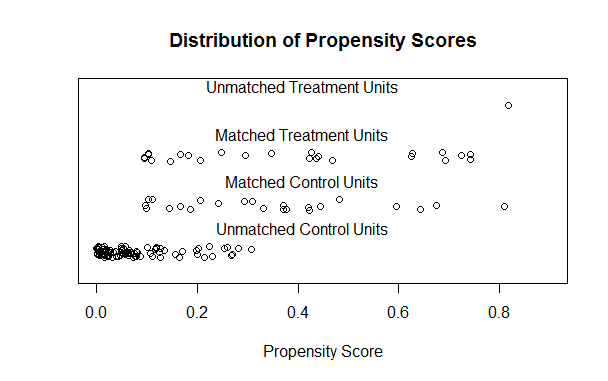
\includegraphics{Jitter}
    \caption{Propensity Score Matching: Jitter Plot}
    \label{Fig1}
\end{figure}

\begin{figure}[h]
    \centering
    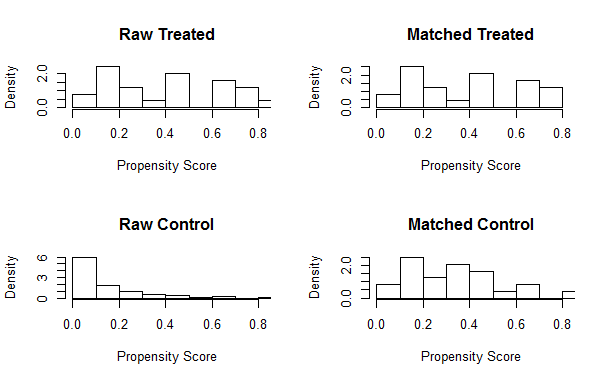
\includegraphics{PSMatch}
    \caption{Propensity Score Matching: Histogram}
    \label{Fig2}
\end{figure}

% Table created by stargazer v.5.2 by Marek Hlavac, Harvard University. E-mail: hlavac at fas.harvard.edu
% Date and time: Wed, Jul 13, 2016 - 11:54:54 AM
\begin{table}[!htbp] \centering 
  \caption{Summary Statistics in 2005 - With PS Matched Control Group} 
  \label{} 
\begin{tabular}{@{\extracolsep{5pt}} ccc} 
\\[-1.8ex]\hline 
\hline \\[-1.8ex] 
 & Undivided & Divided \\ 
\hline \\[-1.8ex] 
TotalMarks & $308.0$ & $302.0$ \\ 
Rural & $0.9$ & $0.9$ \\ 
WorkDays & $90.0$ & $102.0$ \\ 
AcadInsp & $0.5$ & $0.4$ \\ 
DevGrantR & $2,659.0$ & $2,608.0$ \\ 
DevGrantE & $1,470.0$ & $1,279.0$ \\ 
TLMGrantR & $3,585.0$ & $4,007.0$ \\ 
TLMGrantE & $1,966.0$ & $1,777.0$ \\ 
Classrooms & $3.7$ & $3.5$ \\ 
ToiletG & $1$ & $1$ \\ 
Electricity & $0.6$ & $0.5$ \\ 
Library & $0.8$ & $0.8$ \\ 
PlayGround & $0.5$ & $0.5$ \\ 
Male\_Tch & $2.3$ & $2.0$ \\ 
Female\_Tch & $1.7$ & $1.7$ \\ 
Grad\_Tch & $26.0$ & $26.0$ \\ 
ProfQ\_Tch & $3.8$ & $3.3$ \\ 
Days\_nonTch & $1.5$ & $1.8$ \\ 
Public & $0.9$ & $0.9$ \\ 
Split & $0$ & $1$ \\ 
Households & $42,187.0$ & $47,476.0$ \\ 
TotPop & $220,056.0$ & $250,669.0$ \\ 
Pop0.6 & $31,895.0$ & $36,710.0$ \\ 
Literates & $111,360.0$ & $122,912.0$ \\ 
TotWPop & $101,262.0$ & $118,593.0$ \\ 
SCST & $66,376.0$ & $75,755.0$ \\ 
Yr2005 & $299.0$ & $332.0$ \\ 
SchoolperPop2005 & $1.5$ & $1.4$ \\ 
\hline \\[-1.8ex] 
\multicolumn{3}{l}{Population figures used to calculate SchoolperPop2005 is from 2001} \\ 
\end{tabular} 
\end{table} % Table created by stargazer v.5.2 by Marek Hlavac, Harvard University. E-mail: hlavac at fas.harvard.edu
% Date and time: Wed, Jul 13, 2016 - 11:54:54 AM
\begin{table}[!htbp] \centering 
  \caption{Summary Statistics in 2005 - With PS Matched Control Group} 
  \label{} 
\begin{tabular}{@{\extracolsep{5pt}} ccccc} 
\\[-1.8ex]\hline 
\hline \\[-1.8ex] 
 & Variables & Old & New & p.value \\ 
\hline \\[-1.8ex] 
1 & Total Marks & $295.0$ & $311.0$ & 0.17 \\ 
2 & Rural/Urban (rural = 1) & $0.9$ & $0.9$ & 0.58 \\ 
3 & Working Days & $102.0$ & $101.0$ & 0.88 \\ 
4 & Academic Inspection & $0.5$ & $0.3$ & 0.14 \\ 
5 & School Dev Grant - R & $2,554.0$ & $2,684.0$ & 0.73 \\ 
6 & School Dev Grant - E & $1,290.0$ & $1,263.0$ & 0.91 \\ 
7 & TLM Grant - R & $4,093.0$ & $3,888.0$ & 0.69 \\ 
8 & TLM Grant - E & $1,872.0$ & $1,644.0$ & 0.48 \\ 
9 & Classrooms & $3.6$ & $3.3$ & 0.22 \\ 
10 & Electricity (Yes = 1) & $0.5$ & $0.5$ & 0.81 \\ 
11 & Library  (Yes = 1) & $0.8$ & $0.7$ & 0.56 \\ 
12 & PlayGround  (Yes = 1) & $0.5$ & $0.5$ & 0.73 \\ 
13 & Male teachers & $2.0$ & $2.0$ & 0.93 \\ 
14 & Female teachers & $1.8$ & $1.4$ & 0.03 \\ 
15 & Grad teachers & $26.0$ & $26.0$ & 0.97 \\ 
16 & ProfQ teachers & $3.5$ & $3.1$ & 0.08 \\ 
17 & Days\_non teaching activity & $1.5$ & $2.3$ & 0.46 \\ 
18 & Public Schools (\textbackslash \%) & $0.9$ & $0.9$ & 0.8 \\ 
19 & Households & $47,435.0$ & $47,534.0$ & 0.99 \\ 
20 & Total Population & $252,924.0$ & $247,512.0$ & 0.88 \\ 
21 & Population 0 - 6 & $36,703.0$ & $36,719.0$ & 1 \\ 
22 & Literates & $131,616.0$ & $110,726.0$ & 0.26 \\ 
23 & Total W Population & $115,871.0$ & $122,404.0$ & 0.68 \\ 
24 & SC/ST Population & $75,410.0$ & $76,238.0$ & 0.95 \\ 
25 & No of Schools in Taluk & $333.0$ & $332.0$ & 0.98 \\ 
26 & Schools per 1000 people & $1.4$ & $1.4$ & 0.6 \\ 
27 & New/Old Dist (New = 1) & $0$ & $1$ & - \\ 
28 & \textbackslash \# of Observations & $14$ & $10$ & - \\ 
\hline \\[-1.8ex] 
\multicolumn{5}{l}{Population figures used to calculate SchoolperPop2005 is from 2001} \\ 
\end{tabular} 
\end{table} 
% Table created by stargazer v.5.2 by Marek Hlavac, Harvard University. E-mail: hlavac at fas.harvard.edu
% Date and time: Wed, Jul 13, 2016 - 11:54:54 AM
\begin{table}[!htbp] \centering 
  \caption{Summary Statistics in 2013 - With PS Matched Control Group} 
  \label{} 
\begin{tabular}{@{\extracolsep{5pt}} ccc} 
\\[-1.8ex]\hline 
\hline \\[-1.8ex] 
 & Undivided & Divided \\ 
\hline \\[-1.8ex] 
TotalMarks & $333.0$ & $340.0$ \\ 
Rural & $0.9$ & $0.9$ \\ 
WorkDays & $0.7$ & $0.9$ \\ 
AcadInsp & $1.4$ & $1.4$ \\ 
DevGrantR & $8,057.0$ & $7,383.0$ \\ 
DevGrantE & $7,440.0$ & $6,503.0$ \\ 
TLMGrantR & $1,427.0$ & $1,238.0$ \\ 
TLMGrantE & $1,384.0$ & $1,148.0$ \\ 
Classrooms & $4.8$ & $4.7$ \\ 
ToiletG & $1.0$ & $1.0$ \\ 
Electricity & $1.0$ & $1.0$ \\ 
Library & $1.0$ & $1.1$ \\ 
PlayGround & $0.6$ & $0.6$ \\ 
Male\_Tch & $2.1$ & $2.1$ \\ 
Female\_Tch & $2.0$ & $2.1$ \\ 
Grad\_Tch & $0.9$ & $0.9$ \\ 
ProfQ\_Tch & $4.1$ & $4.1$ \\ 
Days\_nonTch & $0.2$ & $0.3$ \\ 
Public & $0.9$ & $0.8$ \\ 
Split & $0$ & $1$ \\ 
Households & $44,302.0$ & $46,508.0$ \\ 
TotPop & $209,137.0$ & $227,783.0$ \\ 
Pop0.6 & $25,456.0$ & $28,933.0$ \\ 
Literates & $123,107.0$ & $125,461.0$ \\ 
TotWPop & $103,334.0$ & $113,280.0$ \\ 
SCST & $72,192.0$ & $77,860.0$ \\ 
Yr2013 & $318.0$ & $367.0$ \\ 
SchoolperPop2013 & $1.7$ & $1.7$ \\ 
\hline \\[-1.8ex] 
\multicolumn{3}{l}{Population figures used to calculate SchoolperPop2013 is from 2001} \\ 
\end{tabular} 
\end{table} % Table created by stargazer v.5.2 by Marek Hlavac, Harvard University. E-mail: hlavac at fas.harvard.edu
% Date and time: Wed, Jul 13, 2016 - 11:54:54 AM
\begin{table}[!htbp] \centering 
  \caption{Summary Statistics in 2013 - With PS Matched Control Group} 
  \label{} 
\begin{tabular}{@{\extracolsep{5pt}} ccccc} 
\\[-1.8ex]\hline 
\hline \\[-1.8ex] 
 & Variables & Old & New & p.value \\ 
\hline \\[-1.8ex] 
1 & Total Marks & $344.0$ & $333.0$ & 0.33 \\ 
2 & Rural/Urban (rural = 1) & $0.9$ & $0.9$ & 0.56 \\ 
3 & Working Days & $0.7$ & $1.1$ & 0.57 \\ 
4 & Academic Inspection & $1.3$ & $1.6$ & 0.67 \\ 
5 & School Dev Grant - R & $7,260.0$ & $7,574.0$ & 0.6 \\ 
6 & School Dev Grant - E & $6,542.0$ & $6,442.0$ & 0.76 \\ 
7 & TLM Grant - R & $1,098.0$ & $1,456.0$ & 0.19 \\ 
8 & TLM Grant - E & $1,017.0$ & $1,352.0$ & 0.18 \\ 
9 & Classrooms & $4.9$ & $4.5$ & 0.2 \\ 
10 & Electricity (Yes = 1) & $1.0$ & $1.0$ & 0.62 \\ 
11 & Library  (Yes = 1) & $1.0$ & $1.2$ & 0.36 \\ 
12 & PlayGround  (Yes = 1) & $0.6$ & $0.5$ & 0.57 \\ 
13 & Male teachers & $2.1$ & $2.1$ & 0.94 \\ 
14 & Female teachers & $2.4$ & $1.8$ & 0 \\ 
15 & Grad teachers & $1.0$ & $0.7$ & 0.21 \\ 
16 & ProfQ teachers & $4.4$ & $3.7$ & 0.03 \\ 
17 & Days\_non teaching activity & $0.5$ & $0.1$ & 0.2 \\ 
18 & Public Schools (\textbackslash \%) & $0.8$ & $0.9$ & 0.18 \\ 
19 & Households & $45,379.0$ & $48,264.0$ & 0.66 \\ 
20 & Total Population & $222,491.0$ & $236,014.0$ & 0.7 \\ 
21 & Population 0 - 6 & $27,863.0$ & $30,597.0$ & 0.69 \\ 
22 & Literates & $129,369.0$ & $119,382.0$ & 0.53 \\ 
23 & Total W Population & $108,226$ & $121,141$ & 0.44 \\ 
24 & SC/ST Population & $73,461.0$ & $84,702$ & 0.45 \\ 
25 & No of Schools in Taluk & $333.0$ & $337.0$ & 0.93 \\ 
26 & Schools per 1000 people & $1.5$ & $1.6$ & 0.77 \\ 
27 & New/Old Dist (New = 1) & $0$ & $1$ & - \\ 
28 & \textbackslash \# of Observations & $14$ & $9$ & - \\ 
\hline \\[-1.8ex] 
\multicolumn{5}{l}{Population figures used to calculate SchoolperPop2013 is from 2001} \\ 
\end{tabular} 
\end{table} \clearpage
% Table created by stargazer v.5.2 by Marek Hlavac, Harvard University. E-mail: hlavac at fas.harvard.edu
% Date and time: Wed, Jul 13, 2016 - 11:54:54 AM
\begin{table}[!htbp] \centering 
  \caption{} 
  \label{} 
\begin{tabular}{@{\extracolsep{5pt}}lcccc} 
\\[-1.8ex]\hline 
\hline \\[-1.8ex] 
 & \multicolumn{4}{c}{\textit{Dependent variable:}} \\ 
\cline{2-5} 
\\[-1.8ex] & SchoolNo & Public & DevGrantR & TLMGrantR \\ 
\\[-1.8ex] & (1) & (2) & (3) & (4)\\ 
\hline \\[-1.8ex] 
 Split & 0.1 & 0.000 & $-$91.0 & 278.0 \\ 
  & (0.1) & (0.02) & (304.0) & (364.0) \\ 
  & & & & \\ 
 Post & 0.2$^{**}$ & $-$0.1$^{***}$ & 5,754.0$^{***}$ & $-$1,750.0$^{***}$ \\ 
  & (0.1) & (0.02) & (319.0) & (383.0) \\ 
  & & & & \\ 
 Literacy & $-$0.01$^{*}$ & $-$0.003$^{**}$ & 9.4 & $-$36.0 \\ 
  & (0.01) & (0.001) & (22.0) & (26.0) \\ 
  & & & & \\ 
 YoungPop & 0.03 & $-$0.02$^{***}$ & 172.0$^{**}$ & 42.0 \\ 
  & (0.02) & (0.004) & (85.0) & (102.0) \\ 
  & & & & \\ 
 Split:Post & $-$0.03 & $-$0.02 & $-$667.0 & $-$672.0 \\ 
  & (0.1) & (0.02) & (426.0) & (511.0) \\ 
  & & & & \\ 
 Constant & 0.1 & 1.4$^{***}$ & $-$248.0 & 4,900.0$^{*}$ \\ 
  & (0.5) & (0.1) & (2,290.0) & (2,748.0) \\ 
  & & & & \\ 
\hline \\[-1.8ex] 
Observations & 95 & 95 & 95 & 95 \\ 
R$^{2}$ & 0.3 & 0.4 & 0.9 & 0.5 \\ 
Adjusted R$^{2}$ & 0.3 & 0.4 & 0.9 & 0.5 \\ 
Residual Std. Error & 0.2 & 0.1 & 1,037.0 & 1,244.0 \\ 
F Statistic & 8.0$^{***}$ & 11.0$^{***}$ & 118.0$^{***}$ & 21.0$^{***}$ \\ 
\hline 
\hline \\[-1.8ex] 
\textit{Note:}  & \multicolumn{4}{r}{$^{*}$p$<$0.1; $^{**}$p$<$0.05; $^{***}$p$<$0.01} \\ 
\end{tabular} 
\end{table} % Table created by stargazer v.5.2 by Marek Hlavac, Harvard University. E-mail: hlavac at fas.harvard.edu
% Date and time: Wed, Jul 13, 2016 - 11:54:55 AM
\begin{table}[!htbp] \centering 
  \caption{} 
  \label{} 
\begin{tabular}{@{\extracolsep{5pt}}lcccc} 
\\[-1.8ex]\hline 
\hline \\[-1.8ex] 
 & \multicolumn{4}{c}{\textit{Dependent variable:}} \\ 
\cline{2-5} 
\\[-1.8ex] & Classrooms & ToiletG & Electricity & Library \\ 
\\[-1.8ex] & (1) & (2) & (3) & (4)\\ 
\hline \\[-1.8ex] 
 Split & $-$0.3 & $-$0.001 & $-$0.04 & $-$0.01 \\ 
  & (0.2) & (0.001) & (0.04) & (0.1) \\ 
  & & & & \\ 
 Post & $-$0.1 & $-$0.01$^{***}$ & 0.3$^{***}$ & 0.1 \\ 
  & (0.4) & (0.003) & (0.1) & (0.2) \\ 
  & & & & \\ 
 SchoolNo & 0.04 & 0.01$^{***}$ & $-$0.01 & $-$0.1 \\ 
  & (0.3) & (0.002) & (0.1) & (0.1) \\ 
  & & & & \\ 
 Public & $-$11.0$^{***}$ & 0.005 & $-$0.6$^{**}$ & 0.4 \\ 
  & (1.2) & (0.01) & (0.3) & (0.6) \\ 
  & & & & \\ 
 DevGrantR & 0.000$^{***}$ & 0.000$^{**}$ & 0.000 & 0.000 \\ 
  & (0.000) & (0.000) & (0.000) & (0.000) \\ 
  & & & & \\ 
 TLMGrantR & 0.000$^{**}$ & $-$0.000 & 0.000 & 0.000 \\ 
  & (0.000) & (0.000) & (0.000) & (0.000) \\ 
  & & & & \\ 
 Literacy & 0.001 & $-$0.000 & 0.004 & $-$0.01 \\ 
  & (0.01) & (0.000) & (0.003) & (0.01) \\ 
  & & & & \\ 
 YoungPop & 0.03 & $-$0.001$^{**}$ & $-$0.01 & $-$0.04 \\ 
  & (0.1) & (0.000) & (0.01) & (0.03) \\ 
  & & & & \\ 
 Split:Post & 0.1 & 0.004$^{*}$ & 0.1 & 0.2 \\ 
  & (0.2) & (0.002) & (0.05) & (0.1) \\ 
  & & & & \\ 
 Constant & 12.0$^{***}$ & 1.0$^{***}$ & 1.0$^{**}$ & 1.2 \\ 
  & (2.1) & (0.02) & (0.4) & (1.0) \\ 
  & & & & \\ 
\hline \\[-1.8ex] 
Observations & 95 & 95 & 95 & 95 \\ 
R$^{2}$ & 0.8 & 0.4 & 0.8 & 0.3 \\ 
Adjusted R$^{2}$ & 0.8 & 0.3 & 0.8 & 0.2 \\ 
Residual Std. Error & 0.6 & 0.004 & 0.1 & 0.3 \\ 
F Statistic & 34.0$^{***}$ & 6.5$^{***}$ & 35.0$^{***}$ & 3.8$^{***}$ \\ 
\hline 
\hline \\[-1.8ex] 
\textit{Note:}  & \multicolumn{4}{r}{$^{*}$p$<$0.1; $^{**}$p$<$0.05; $^{***}$p$<$0.01} \\ 
\end{tabular} 
\end{table} % Table created by stargazer v.5.2 by Marek Hlavac, Harvard University. E-mail: hlavac at fas.harvard.edu
% Date and time: Wed, Jul 13, 2016 - 11:54:55 AM
\begin{table}[!htbp] \centering 
  \caption{} 
  \label{} 
\begin{tabular}{@{\extracolsep{5pt}}lcccc} 
\\[-1.8ex]\hline 
\hline \\[-1.8ex] 
 & \multicolumn{4}{c}{\textit{Dependent variable:}} \\ 
\cline{2-5} 
\\[-1.8ex] & Male\_Tch & Female\_Tch & Grad\_Tch & ProfQ\_Tch \\ 
\\[-1.8ex] & (1) & (2) & (3) & (4)\\ 
\hline \\[-1.8ex] 
 Split & $-$0.4$^{***}$ & 0.1 & 0.8 & $-$0.5$^{***}$ \\ 
  & (0.1) & (0.1) & (4.6) & (0.2) \\ 
  & & & & \\ 
 Post & $-$0.3 & $-$0.2 & $-$8.8 & $-$0.04 \\ 
  & (0.3) & (0.3) & (12.0) & (0.5) \\ 
  & & & & \\ 
 SchoolNo & 1.0$^{***}$ & $-$0.8$^{***}$ & $-$23.0$^{***}$ & 0.04 \\ 
  & (0.2) & (0.2) & (7.4) & (0.3) \\ 
  & & & & \\ 
 Public & $-$2.1$^{**}$ & $-$8.1$^{***}$ & 11.0 & $-$8.5$^{***}$ \\ 
  & (1.0) & (1.0) & (33.0) & (1.3) \\ 
  & & & & \\ 
 DevGrantR & 0.000 & 0.000 & $-$0.002 & 0.000 \\ 
  & (0.000) & (0.000) & (0.002) & (0.000) \\ 
  & & & & \\ 
 TLMGrantR & 0.000 & 0.000 & 0.000 & 0.000 \\ 
  & (0.000) & (0.000) & (0.001) & (0.000) \\ 
  & & & & \\ 
 Literacy & 0.02 & 0.001 & $-$0.2 & 0.02 \\ 
  & (0.01) & (0.01) & (0.3) & (0.01) \\ 
  & & & & \\ 
 YoungPop & 0.1$^{***}$ & $-$0.04 & 1.3 & 0.1$^{**}$ \\ 
  & (0.04) & (0.05) & (1.5) & (0.1) \\ 
  & & & & \\ 
 Split:Post & 0.3 & 0.03 & $-$1.7 & 0.4 \\ 
  & (0.2) & (0.2) & (6.5) & (0.3) \\ 
  & & & & \\ 
 Constant & 1.2 & 9.3$^{***}$ & 16.0 & 8.1$^{***}$ \\ 
  & (1.6) & (1.7) & (57.0) & (2.3) \\ 
  & & & & \\ 
\hline \\[-1.8ex] 
Observations & 95 & 95 & 95 & 95 \\ 
R$^{2}$ & 0.6 & 0.6 & 0.5 & 0.6 \\ 
Adjusted R$^{2}$ & 0.6 & 0.6 & 0.4 & 0.6 \\ 
Residual Std. Error & 0.4 & 0.5 & 16.0 & 0.6 \\ 
F Statistic & 15.0$^{***}$ & 18.0$^{***}$ & 8.5$^{***}$ & 16.0$^{***}$ \\ 
\hline 
\hline \\[-1.8ex] 
\textit{Note:}  & \multicolumn{4}{r}{$^{*}$p$<$0.1; $^{**}$p$<$0.05; $^{***}$p$<$0.01} \\ 
\end{tabular} 
\end{table} % Table created by stargazer v.5.2 by Marek Hlavac, Harvard University. E-mail: hlavac at fas.harvard.edu
% Date and time: Wed, Jul 13, 2016 - 11:54:55 AM
\begin{table}[!htbp] \centering 
  \caption{} 
  \label{} 
\begin{tabular}{@{\extracolsep{5pt}}lcccc} 
\\[-1.8ex]\hline 
\hline \\[-1.8ex] 
 & \multicolumn{4}{c}{\textit{Dependent variable:}} \\ 
\cline{2-5} 
\\[-1.8ex] & WorkDays & Days\_nonTch & AcadInsp & TotalMarks \\ 
\\[-1.8ex] & (1) & (2) & (3) & (4)\\ 
\hline \\[-1.8ex] 
 Split & 11.0$^{***}$ & 0.6 & $-$0.1 & $-$3.6 \\ 
  & (4.2) & (0.6) & (0.3) & (7.2) \\ 
  & & & & \\ 
 Post & $-$114.0$^{***}$ & $-$4.6$^{***}$ & $-$0.03 & 12.0 \\ 
  & (11.0) & (1.5) & (0.7) & (19.0) \\ 
  & & & & \\ 
 SchoolNo & 0.9 & $-$0.7 & 0.3 & $-$24.0$^{**}$ \\ 
  & (6.8) & (0.9) & (0.4) & (12.0) \\ 
  & & & & \\ 
 Public & $-$43.0 & $-$1.6 & $-$4.6$^{**}$ & $-$18.0 \\ 
  & (30.0) & (4.2) & (1.9) & (52.0) \\ 
  & & & & \\ 
 DevGrantR & 0.004$^{**}$ & 0.000 & 0.000 & 0.000 \\ 
  & (0.002) & (0.000) & (0.000) & (0.003) \\ 
  & & & & \\ 
 TLMGrantR & 0.000 & $-$0.001$^{***}$ & $-$0.000 & $-$0.002 \\ 
  & (0.001) & (0.000) & (0.000) & (0.002) \\ 
  & & & & \\ 
 Literacy & $-$0.6$^{*}$ & $-$0.03 & $-$0.02 & $-$0.5 \\ 
  & (0.3) & (0.04) & (0.02) & (0.5) \\ 
  & & & & \\ 
 YoungPop & $-$3.2$^{**}$ & $-$0.1 & 0.04 & $-$4.4$^{*}$ \\ 
  & (1.4) & (0.2) & (0.1) & (2.4) \\ 
  & & & & \\ 
 Split:Post & $-$9.8 & $-$0.5 & 0.1 & 13.0 \\ 
  & (6.0) & (0.8) & (0.4) & (10.0) \\ 
  & & & & \\ 
 Constant & 192.0$^{***}$ & 8.4 & 4.9 & 425.0$^{***}$ \\ 
  & (52.0) & (7.2) & (3.2) & (90.0) \\ 
  & & & & \\ 
\hline \\[-1.8ex] 
Observations & 95 & 95 & 95 & 95 \\ 
R$^{2}$ & 0.9 & 0.3 & 0.4 & 0.4 \\ 
Adjusted R$^{2}$ & 0.9 & 0.2 & 0.4 & 0.4 \\ 
Residual Std. Error & 14.0 & 2.0 & 0.9 & 24.0 \\ 
F Statistic & 120.0$^{***}$ & 3.5$^{***}$ & 6.6$^{***}$ & 7.1$^{***}$ \\ 
\hline 
\hline \\[-1.8ex] 
\textit{Note:}  & \multicolumn{4}{r}{$^{*}$p$<$0.1; $^{**}$p$<$0.05; $^{***}$p$<$0.01} \\ 
\end{tabular} 
\end{table} 




\end{document}
